\documentclass[14pt,a4paper]{extreport}

% Caption configuration
\usepackage{caption}

% Times New Roman, be sure to build with XeLaTeX
\usepackage{fontspec}
\usepackage[russian]{babel}
\setmainfont{Times New Roman}

% mock data
\usepackage{lipsum}

% russian
%\usepackage[14pt]{extsizes}
%\usepackage[T2A, T1]{fontenc}
\usepackage[utf8]{inputenc}
%\usepackage{cmap}
%\usepackage{wrapfig}

\linespread{1.5}

\usepackage{graphicx}
\usepackage[
    letterpaper,
    left        = 2cm,
    right       = 1cm,
    top         = 1cm,
    headheight  = 2cm
]{geometry}

% index caption label
\newcommand{\screenshot}[3]{\begin{figure}[ht]%
\centering%
\includegraphics[width=0.8\textwidth]{../screenshots/screen-#1}%
\caption{#2}%
\label{#3}%
\end{figure}%
}

%configurations

% Рис 1. -> Рис 1 --, Таблица 1. -> Таблица 1 --
% Рис 1. -> Рисунок 1
\DeclareCaptionFormat{myformat}{\fontsize{12}{12}\selectfont#1#2#3}
\captionsetup[figure]{format={myformat},name={Рисунок},labelsep=endash}


\begin{document}

	\begin{titlepage}
	\begin{center}	
		\fontsize{14pt}{14pt}\selectfont
		МИНИСТЕРСТВО ОБРАЗОВАНИЯ И НАУКИ\\

		\vspace*{0.6\baselineskip}
		
		САНКТ-ПЕТЕРБУРГСКИЙ НАЦИОНАЛЬНЫЙ ИССЛЕДОВАТЕЛЬСКИЙ УНИВЕРСИТЕТ ИНФОРМАЦИОННЫХ ТЕХНОЛОГИЙ, МЕХАНИКИ И ОПТИКИ
		
		\vspace*{0.6\baselineskip}
		ФАКУЛЬТЕТ ИНФОКОММУНИКАЦИОННЫХ ТЕХНОЛОГИЙ
		КАФЕДРА ПРОГРАММНЫХ СИСТЕМ
	
		\vspace*{7\baselineskip}
		\fontseries{m}\fontsize{19pt}{18pt}\selectfont
		Отчет по лабораторной работе
		
		\fontseries{m}\fontsize{20pt}{18pt}\selectfont
		\textbf{Прослушивание трафика с помощью ПО Wireshark}\\
		\vspace*{1.15\baselineskip}
		\end{center}
	
	\vspace*{2\baselineskip}
	\begin{flushright}
	\fontseries{m}\fontsize{14pt}{14pt}\selectfont
	\textbf{Выполнили:}\\
	Кислюк~И.~В.\\
	Антонов~Е.~П.\\
	Лебедев~И.~Ю.\\
	студенты группы К4120\\
	Проверил: Осипов Н. А.\\
	\end{flushright}
	
	\vspace*{2\baselineskip}
	\begin{center}
	Санкт-Петербург\\
	2017
	\end{center}
	
\end{titlepage}

\newpage

\fontsize{16pt}{14pt}\selectfont
\begin{center}
\textbf{ЦЕЛЬ РАБОТЫ:}
\end{center}

Прослушать трафик с помощью программы WireShark, который будет сгенерирован следующими командами:

\begin{itemize}
\item Команда ping
\item Команда ping для имени сервера. Пример $ping$~$server$
\end{itemize}

\clearpage

%\fontsize{16pt}{16pt}\selectfont
\begin{center}
\textbf{ХОД РАБОТЫ:}
\end{center}

%\fontsize{14pt}{14pt}\selectfont

\begin{enumerate}

\item Выполним команду ping с серверного компьютера на целевую машину линукса. Пример показан на рисунке~\ref{picture1}.

\begin{figure}[ht]
\centering
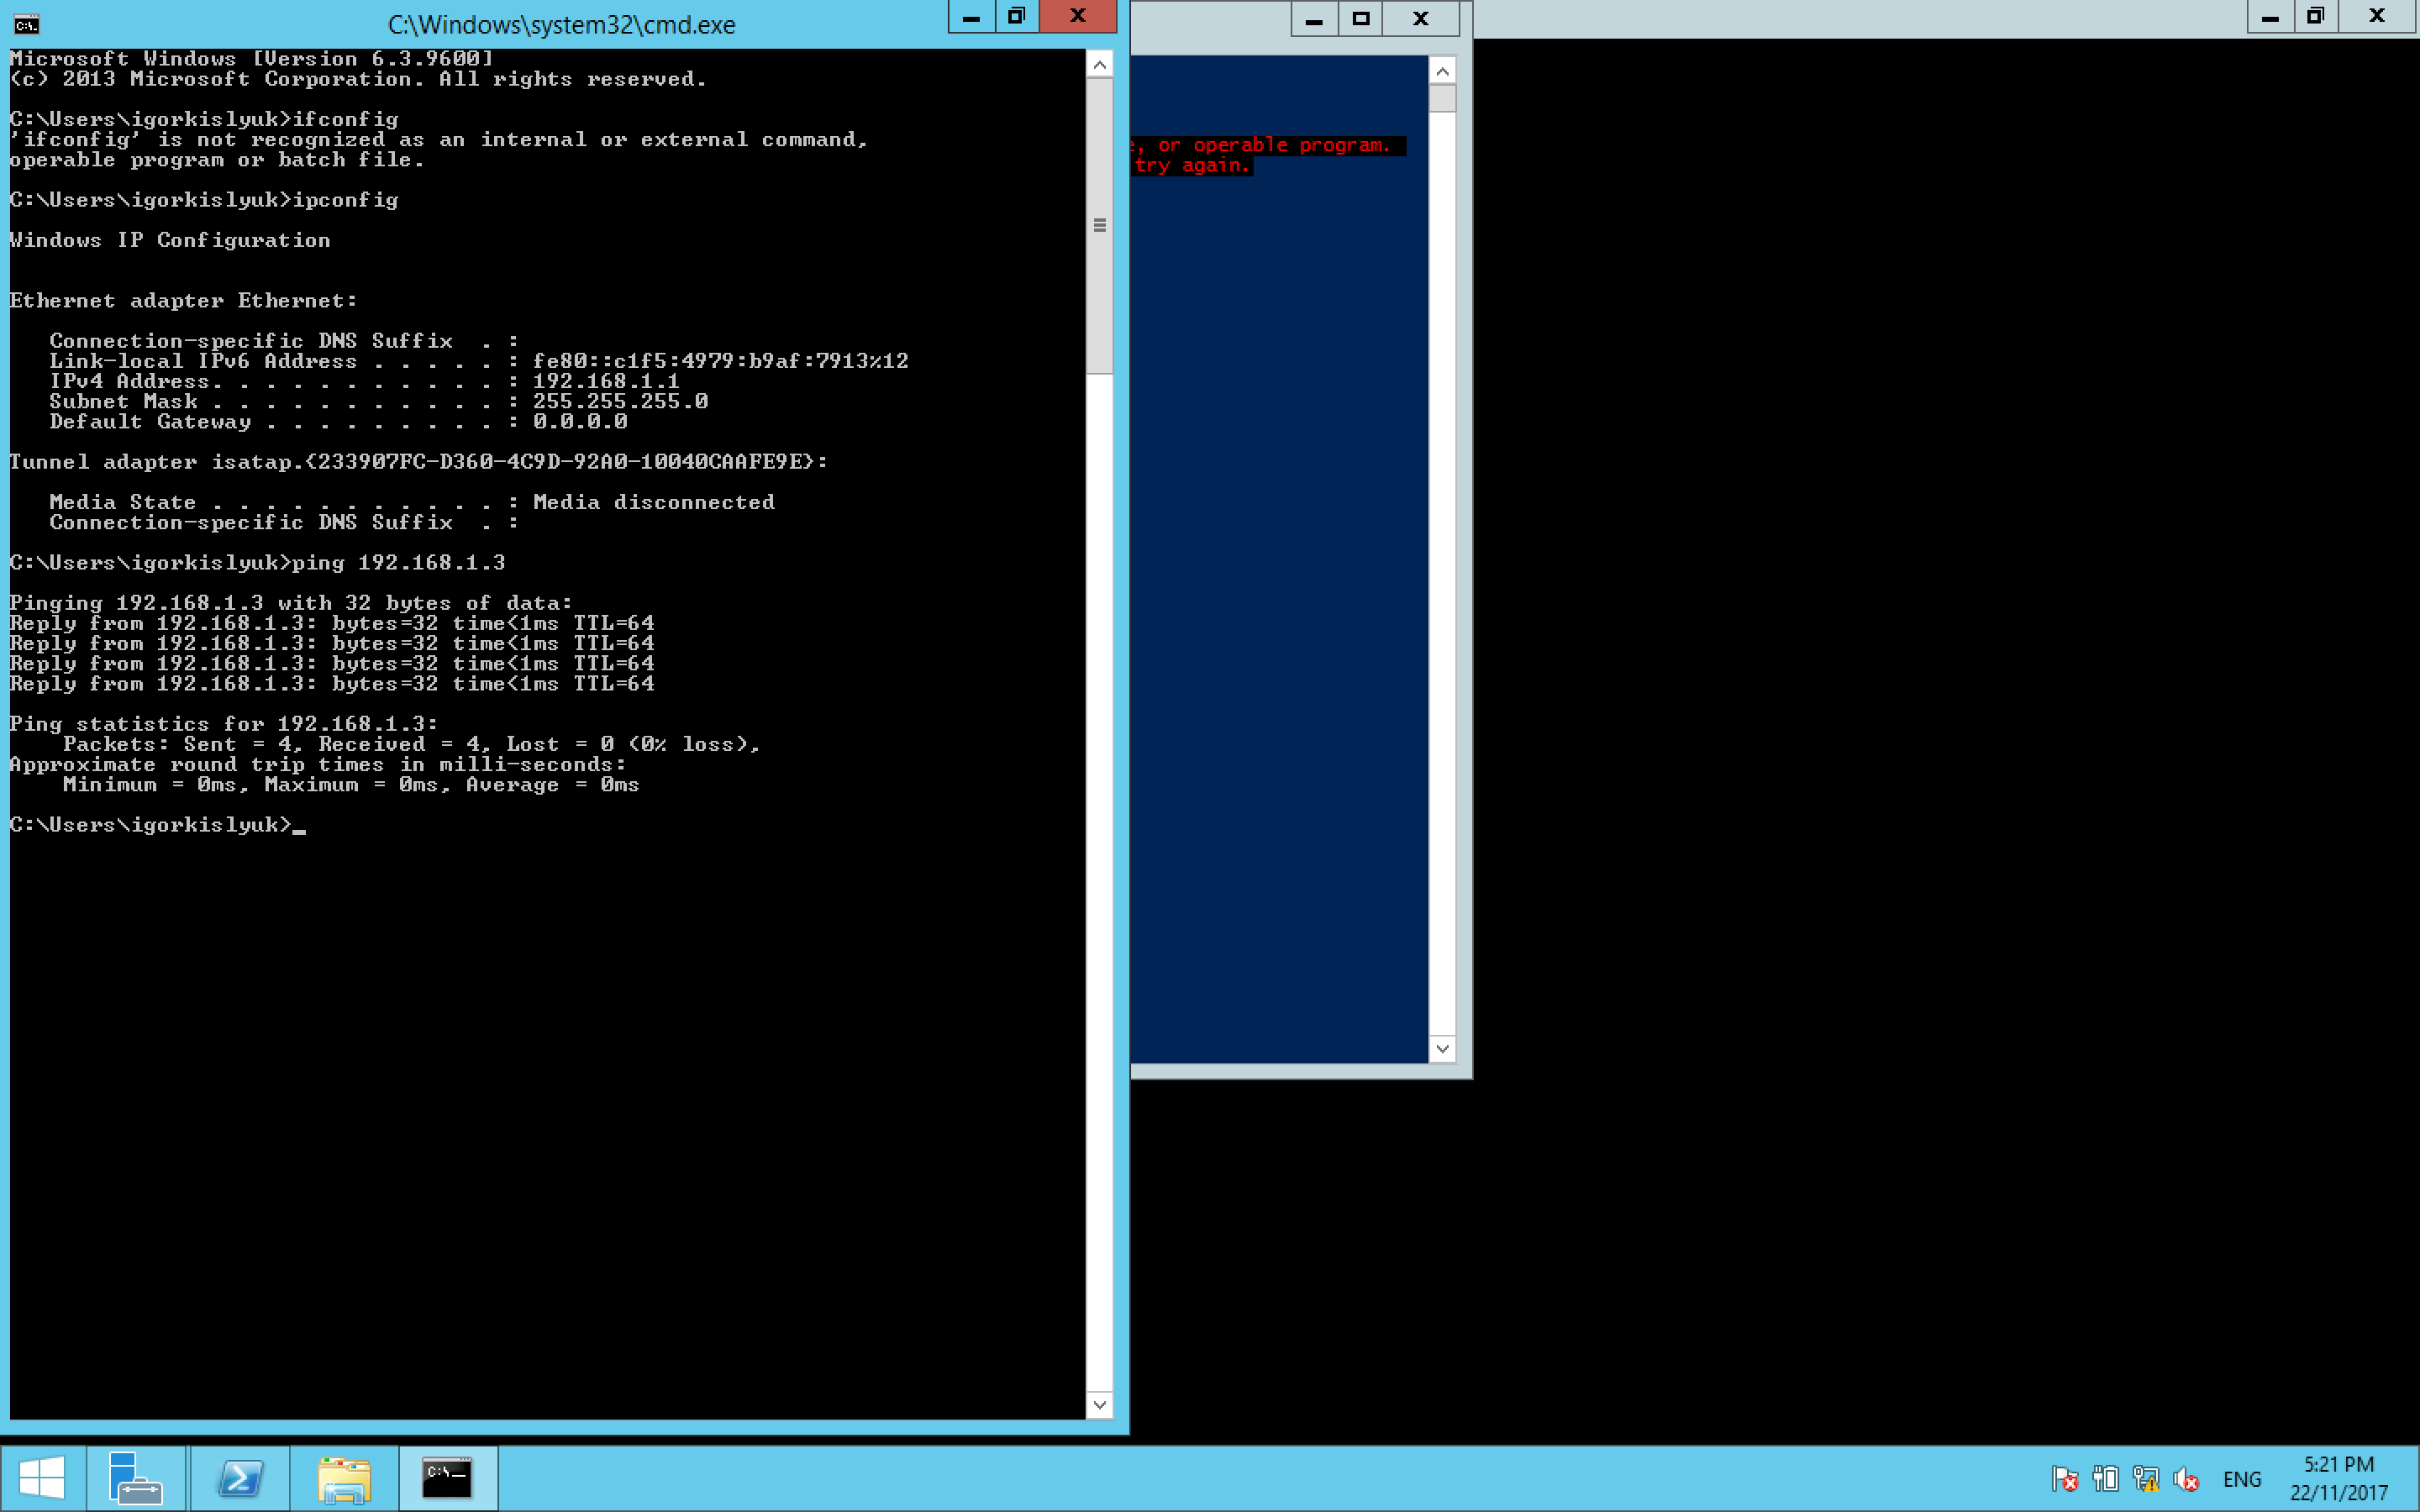
\includegraphics[width=0.8\textwidth]{../screenshots/screen-1}
\caption{Пример интерфейса IContactProvider}
\label{picture1}
\end{figure}

\item Пример команды ping с целевой машины на серверную машину WindowsServer 2012 R2 приведен на рисунке~\ref{picture2}.

\begin{figure}[ht]
\centering
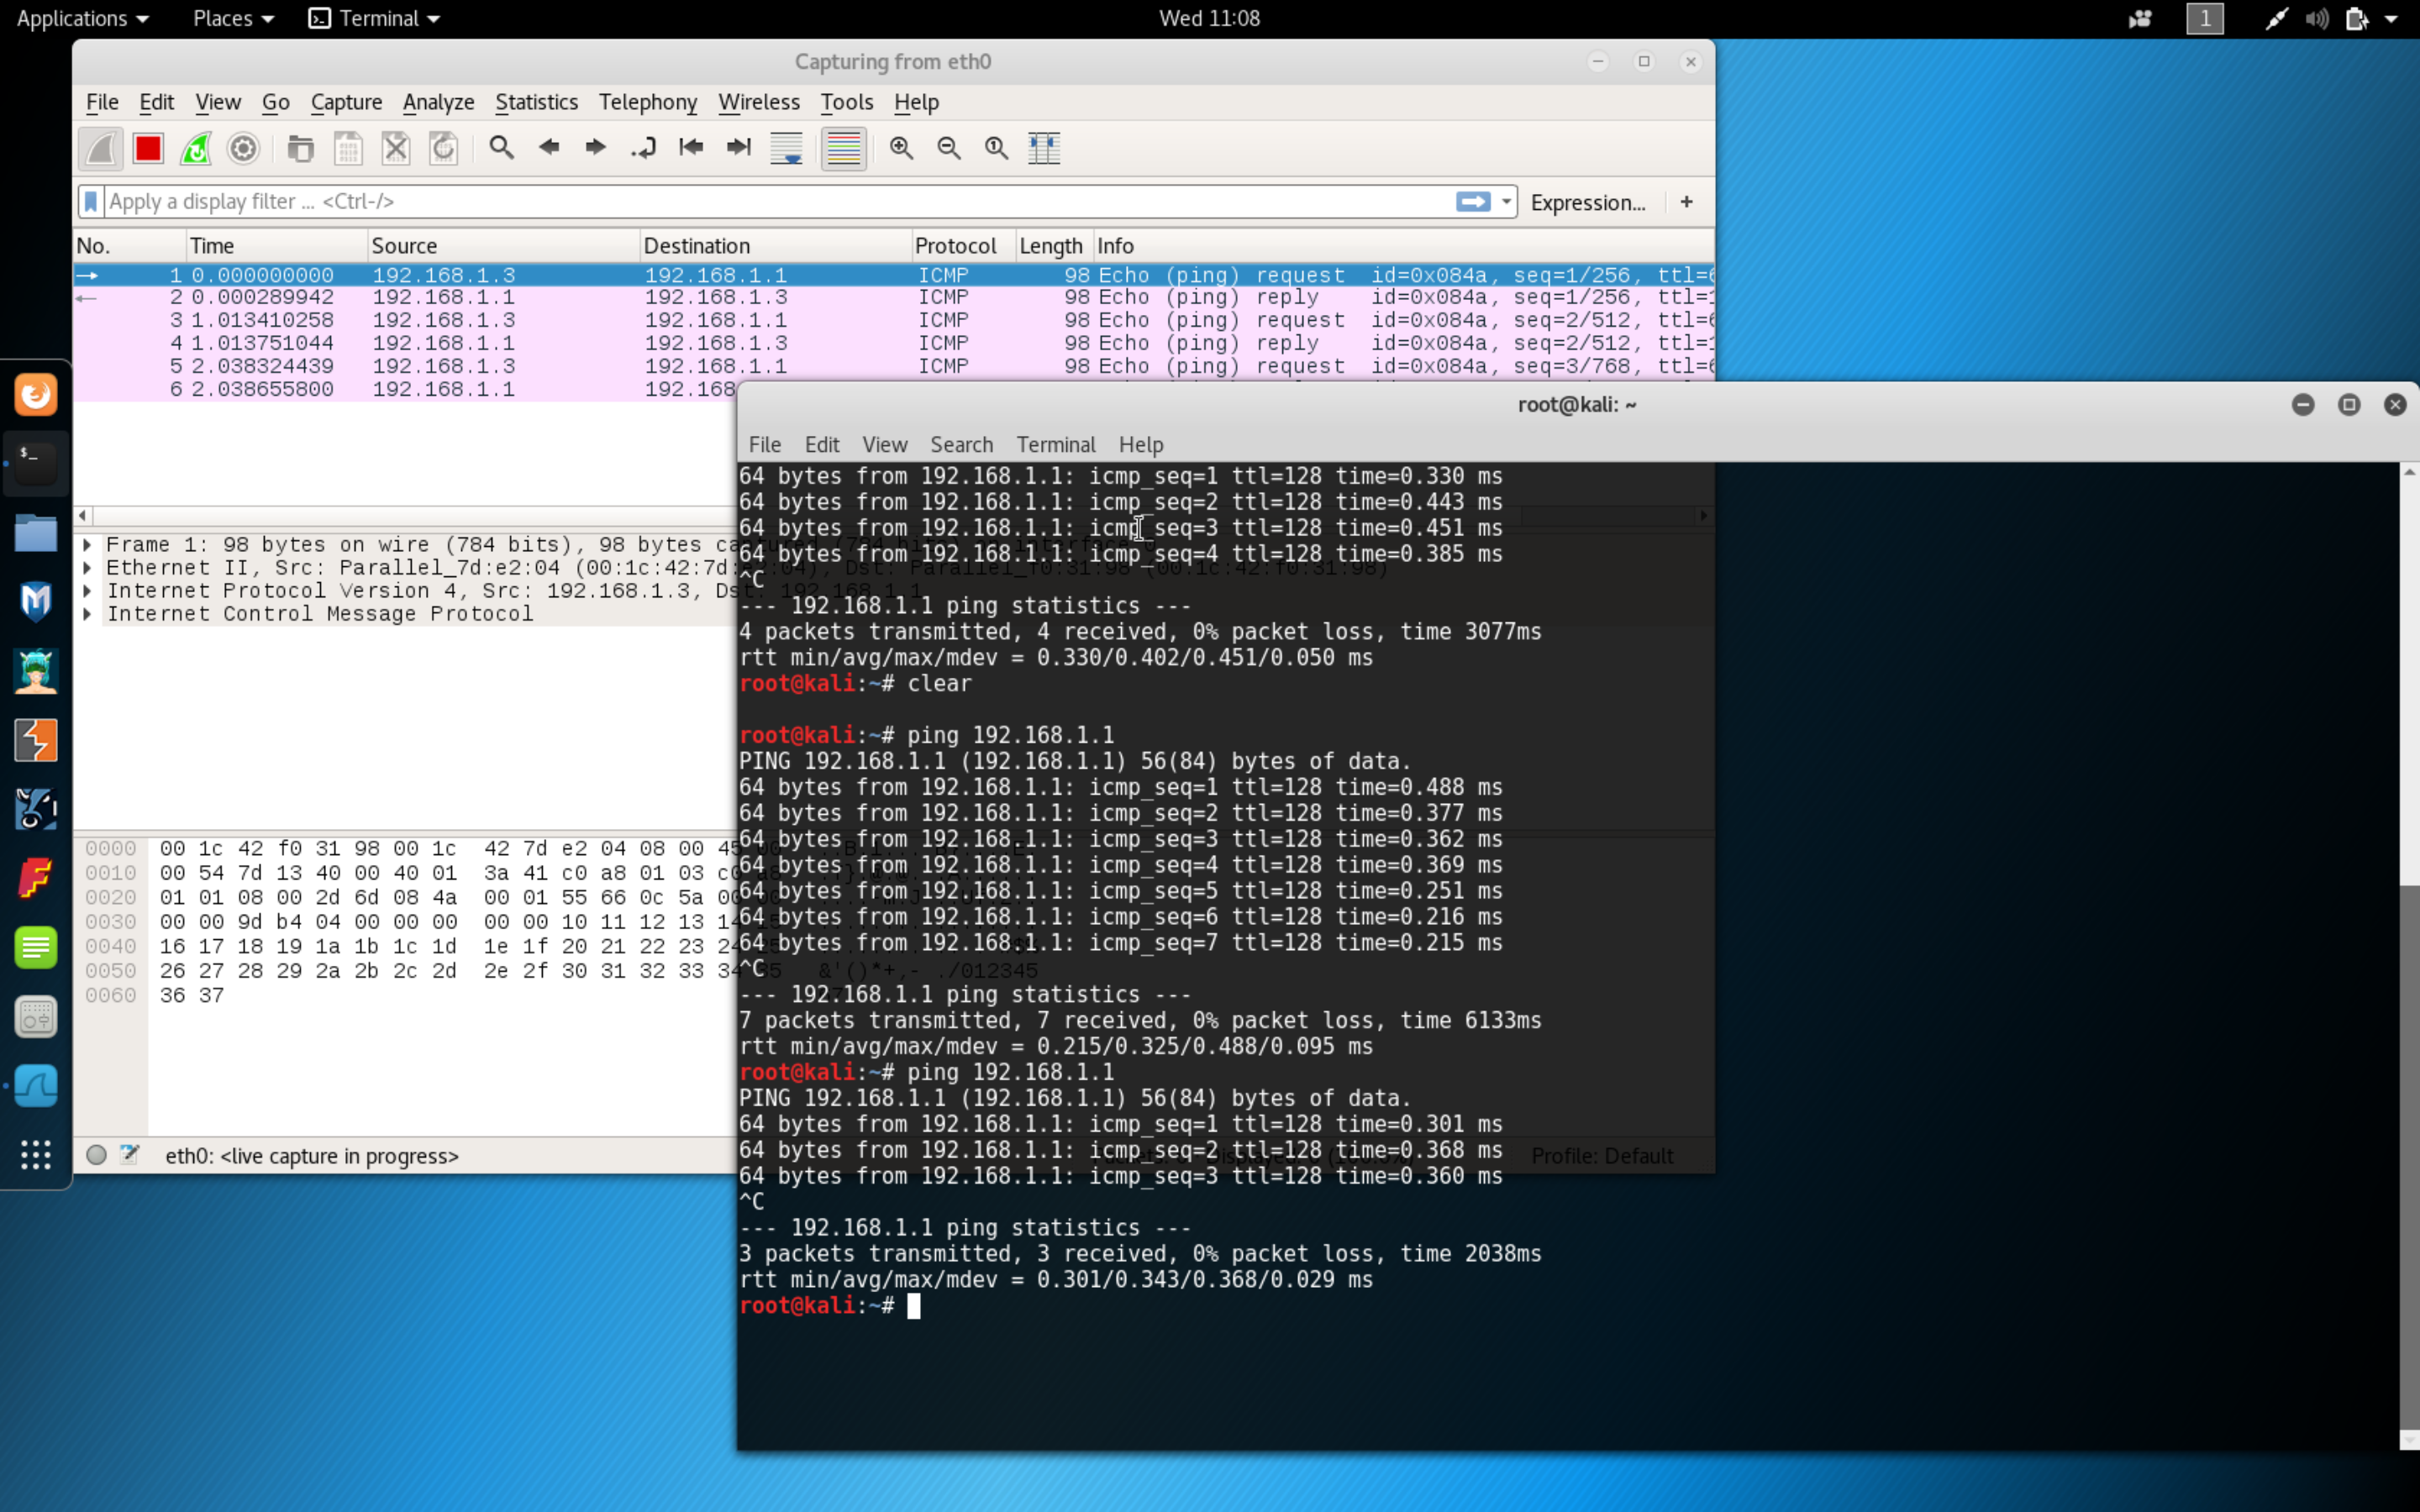
\includegraphics[width=0.8\textwidth]{../screenshots/screen-2}
\caption{Пример реализации сущности Presenter}
\label{picture2}
\end{figure}

\item Пример детального параметров пакета показан на рисунке

\screenshot{3}{Пример деталей для команды ping}{3}

\end{enumerate}

\clearpage

\textbf{Вывод}: таким образом был прослушан трафик для обычного запроса ping и запроса DNS-сервера, который был поднят на WindowsServer 2012.

\end{document}

